\chapter{Implementation of The Data Pipeline}
\section*{Introduction}
\addcontentsline{toc}{section}{Introduction}

This chapter introduces a comprehensive pipeline designed to collect
and process data for our nutrition application. We start by the data
understanding phase, which involves collecting and exploring the data
to identify potential problems. Then, we detail the data preparation
phase, which includes the implementation of an ETL pipeline to clean,
transform, and load the data into a structured format suitable for use by
the recommendation system and the AI assistant. The data is collected
from various European retailers using web scraping techniques that we
will present it with details in a separated section. The collected data is
then cleaned, transformed, and enriched with additional features such as
the Nutri-Score, dietary labels, and other relevant nutritional indicators.
In the final stage, the processed data is embedded and stored in a vector
database to enable efficient semantic search.
\section{Data Understanding}
Following the Business Understanding phase outlined in the first
chapter, we now advance through the remaining CRISP-DM steps.
This section focuses on the Data Understanding phase, which involves
collecting and exploring the data to identify potential problems.

\subsection{Sources}

\par The data used comes mainly from web scraping of a wide variety of
food products in Europe. We scraped data from the websites of major
supermarkets in France, Italy, Germany, and Spain.
The scraped data includes detailed product information and nutritional
values such as calories, carbohydrates, fats, and proteins, as well as
ingredients and allergens.

\begin{center}
\begin{figure}[H]
    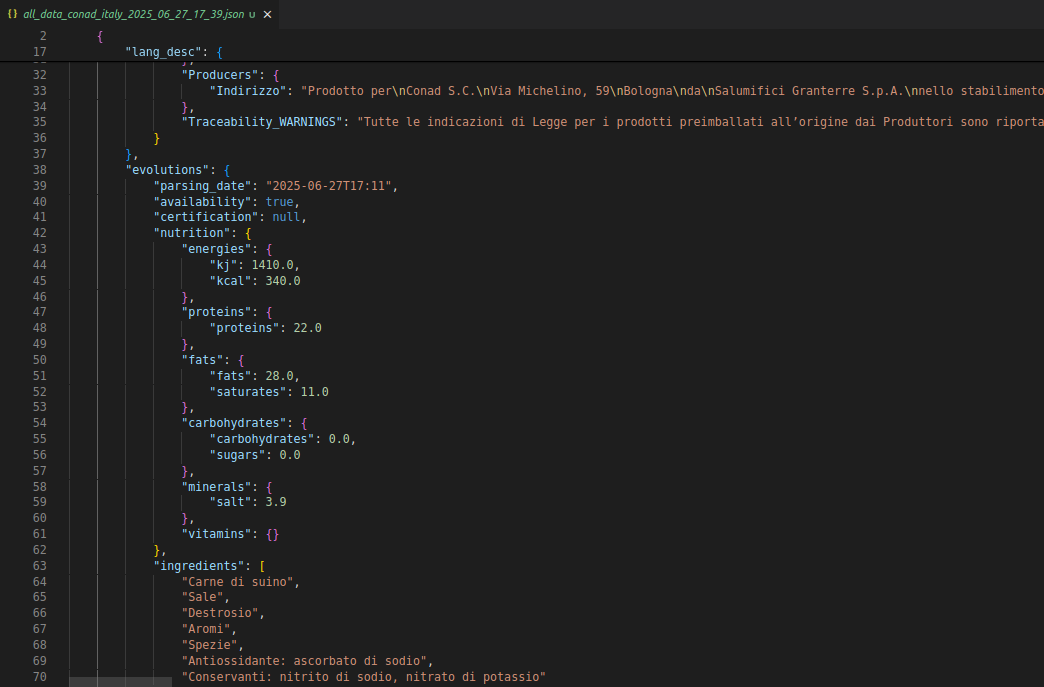
\includegraphics[scale=0.39]{images/conad_italy_data.png}
    \caption{An example of a product details page to scrape from the Italian supermarket chain Esselunga} 
    \label{fig:scraped_data}
\end{figure}
\end{center}


\subsection{Problems} 
The discarded products are diverse and inconsistent, as they come from
several countries and different distributors.
One major challenge in our project is that product descriptions are
written in different languages, which complicates product matching and
recommendation. As shown in Figure 3.1, the product description is in
Italian, while other products have descriptions in French, German, or
Spanish. As a result, we need to implement a multilingual approach
to handle these variations effectively. The descriptions show various
inconsistencies, while essential information, including NutriScore and
nutritional labels, is absent from the data.
As a result, an ETL pipeline is required to collect, process, and unify all
products into a consistent database structure.


\subsection{Data enrichment}
Another challenge is the nutritional evaluation of each product. It is
impractical to manually assess each product by identifying high-sugar
items for individuals with diabetes or detecting products that do not
contain gluten for people with celiac disease. After the web scraping, the
data pipeline must automatically add pertinent health labels and nutrition
indicators like the Nutri-Score in order to solve this problem. This feature
engineering is a crucial step for enabling efficient product filtering and
delivering personalized recommendations. In parallel, data is enriched
with behavioral data from users’ browsing history on the app, including
products viewed, liked, or disliked, as well as user profiles describing their
dietary preferences, allergies, medical conditions or nutritional goals.

\section{Data preparation: ETL pipeline}


The data preparation phase is a crucial step in the CRISP-DM methodology, as it directly impacts the quality and effectiveness of the subsequent
modeling phase. During this phase, we implement an ETL pipeline to
clean, transform, and load the data into a structured format suitable for
use by the recommendation system and the AI assistant. This section
details the technical aspects of the ETL process that was implemented
to collect, process, and integrate products from various European stores,
as well as the tools and methodologies used in this step.

\begin{center}
\begin{figure}[H]
    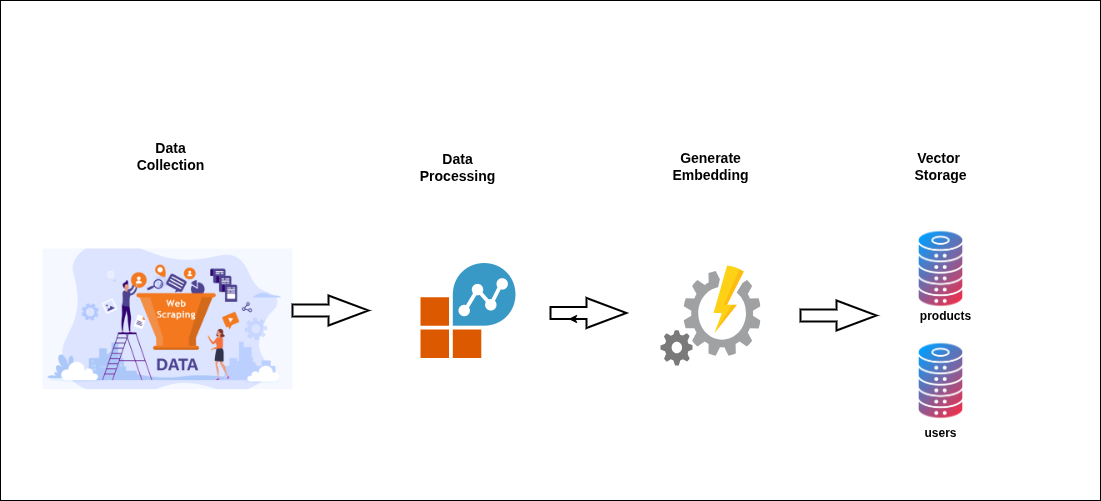
\includegraphics[scale=0.35]{images/workflow__data.png}
    \caption{End-to-end data workflow: from web scraping to vector embedding}
    \label{fig:data_workflow}
\end{figure}
\end{center}

\subsection{Extract}

\par The starting point in the ETL processing workflow is the data extraction phase. It includes gathering nutritional information, prices, and
descriptions from a range retailer websites using web scraping.
\par Despite the variety of websites available in Europe for scraping, there
are many challenges. The retailers websites have different structures and
categories of products. Selecting the appropriate CSS selectors or HTML
tags for each relevant piece of information is therefore a critical step.
These challenges will be examined in greater detail in the subsequent
section on web scraping.
\par The scraped data, as illustrated in Figure \ref{fig:scraped_data}, is initially stored in a raw format as JSON files. This raw data serves as the foundation for subsequent processing and transformation steps.
\begin{center}
\begin{figure}[H]
\centering
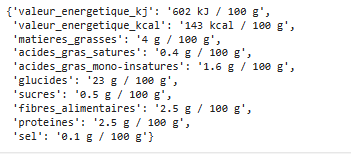
\includegraphics[scale=0.66]{images/nutrition.png}
\caption{Example of a nutrition column before processing} 
\label{fig:Nutrition_column}
\end{figure}
\end{center}

\subsection{Transform}
After that, The gathered data is cleaned, enriched, and standardized
during the transformation phase to guarantee accuracy and compatibility with VitamiNurse’s requirements.
The scraper provided us with comprehensive product information, including many irrelevant columns. We will extract only the relevant product columns to simplify and focus our
analysis.

\subsubsection{Data Cleaning}
We performed a thorough cleaning. To do this, we removed columns
containing products with duplicate EAN codes to eliminate redundancies
and ensure data quality. We also decided to remove columns with
empty nutritional values. Nutritional information was originally located
under the main column "evolutions". We extracted this information and
reorganized it into a separate "nutrition" column, using a dictionary
format.


\subsubsection{Normalization and transformation}

We had to process the "nutrition" column of our database, since it included detailed nutritional information such as energy, fat, carbohydrates,
protein, and salt for each product. For example, here is an entry from
the "nutrition" column.

\begin{center}
\begin{figure}[H]
    \centering
    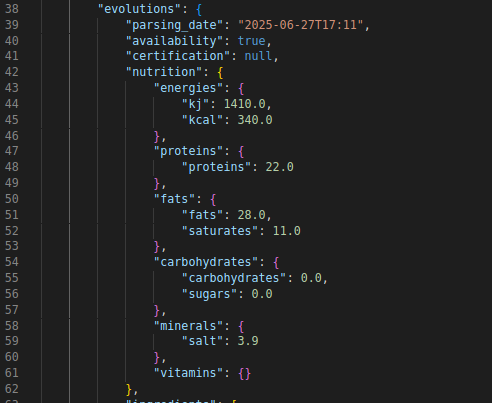
\includegraphics[scale=0.33]{images/transform_nutrition.png}
    \caption{Example of a nutrition column after Normalization and Transformation} 
    \label{fig:Normalization_nutrition}
\end{figure}
\end{center}

\par It was necessary to normalize these data to ensure that they were on
the same scale. Normalization allows feature values to be rescaled so
that they fall within a common range. This is particularly important
for recommendation algorithms, which are sensitive to differences in
magnitude between features.

\par The nutritional values were originally expressed in different units, such as
grams (g), milligrams (mg), and kilocalories (kcal). To ensure consistency,
we converted all nutritional values to a standard unit per 100 grams
of product. As we can see in Figure 3.4, nutrition values are now
standardized per 100g after being scraped from the Conad website. This
standardization allows for direct comparison between products in the
next chapter during the recommendation process.

\subsubsection{Feature engineering}
\par Feature engineering involves creating new features or modifying existing
ones to improve the performance of product evaluation and recommenda-
tion algorithms.

\par As a next step, we constructed a reference dictionary containing specific
keyword lists, such as ingredients that contain gluten, non-vegetarian
components, pork-derived ingredients, and substances to avoid during
pregnancy. These lists are used to generate customized binary features
for each product, enabling the model to make more personalized and
context-sensitive recommendations.

\begin{center}
\begin{figure}[H]
    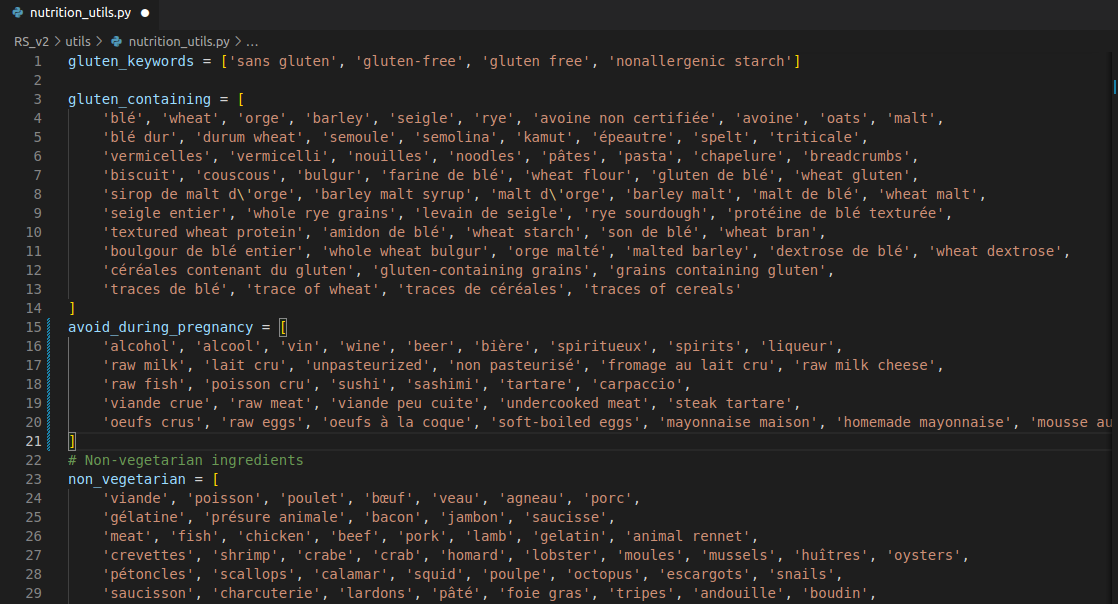
\includegraphics[scale=0.35]{images/nutrition_utils.png}
    \caption{Keywords Dictionary for Automated Nutrition Labelling} 
    \label{fig:nutrition_utils_file}
\end{figure}
\end{center}

After that we combine all the product titles, ingredients, and categories
and check if it matches any specific nutrition to add it. The last step in the
feature engineering process is the computation and assignment of the
Nutri-Score to each product here.
The Nutri-Score is a nutrition label that was first implemented in France
in 2017. It features a five-color scale accompanied by letters from A (most
nutritious) to E (least nutritious). It is designed to provide consumers
with clear and immediate information about the nutritional quality of
food products [12]. As discussed in the Nutri-Score FAQ document [13]
developed by the French Public Health Agency, the system is adapted to
align with dietary guidelines throughout Europe. In the data pipeline,
we implemented a function that automatically calculates the Nutri-Score
for each product based on its nutritional values. This function follows
the official Nutri-Score algorithm, which considers both negative and
positive nutritional factors to determine the final score.

%\begin{center}
%\begin{figure}[H]
%    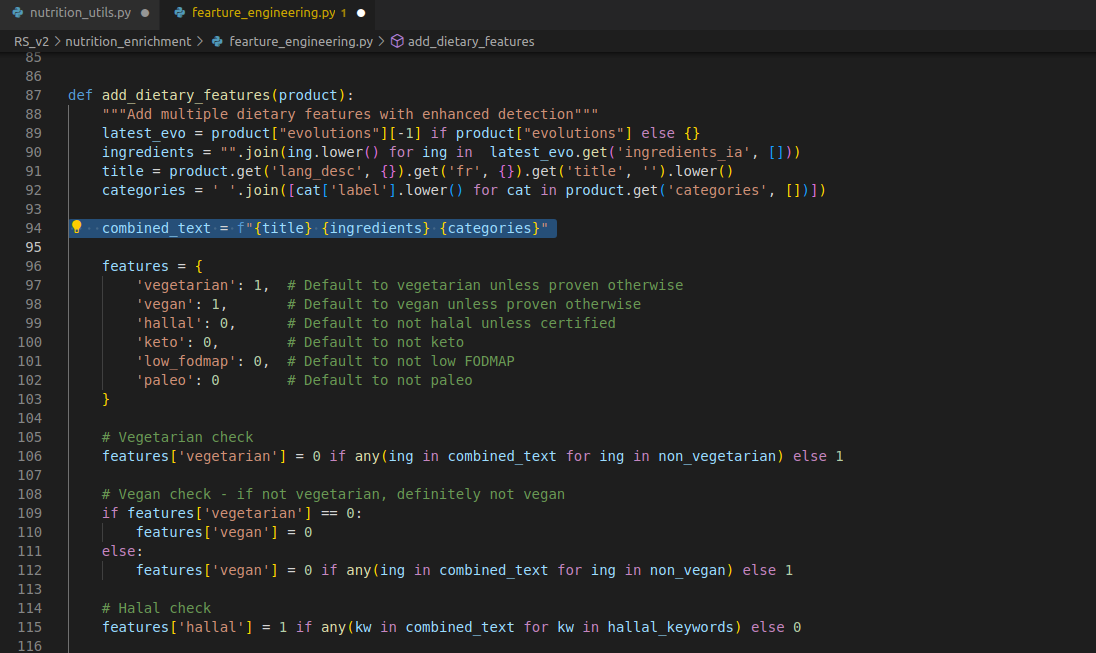
\includegraphics[scale=0.35]{images/feature_engineering.png}
%    \caption{feature engineering} 
%    \label{fig: feature engenieering}
%\end{figure}
%\end{center}


\begin{center}
\begin{figure}[H]
    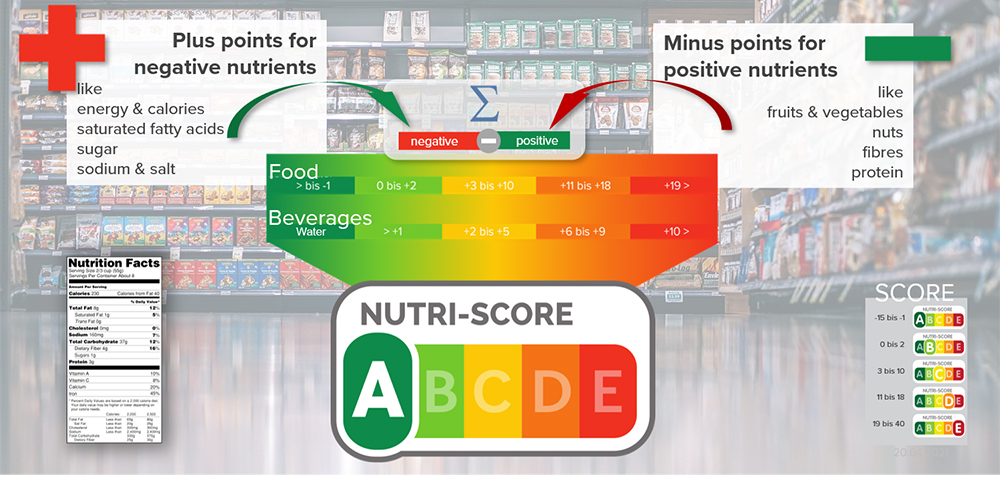
\includegraphics[scale=0.35]{images/nutriscore.jpg}
    \caption{Nutri-Score calculation logic} 
    \label{fig: add_nutriscore}
\end{figure}
\end{center}

\subsection{Load: Data Storage}
After cleaning and transforming the data using an ETL pipeline, the final
phase involves loading the processed information into two complementary
databases to optimize both storage and retrieval.

\subsection{Primary Storage in MongoDB}
As illustrated in Figure\ref{fig:load_data_mongo}, the scraped data are initially stored in MongoDB that serves as the primary database for centralized storage and management. 
This choice guarantees data persistence and reliability, thereby minimizing the risk of data loss while enabling flexible access for subsequent processing stages.


\begin{center}
\begin{figure}[H]
    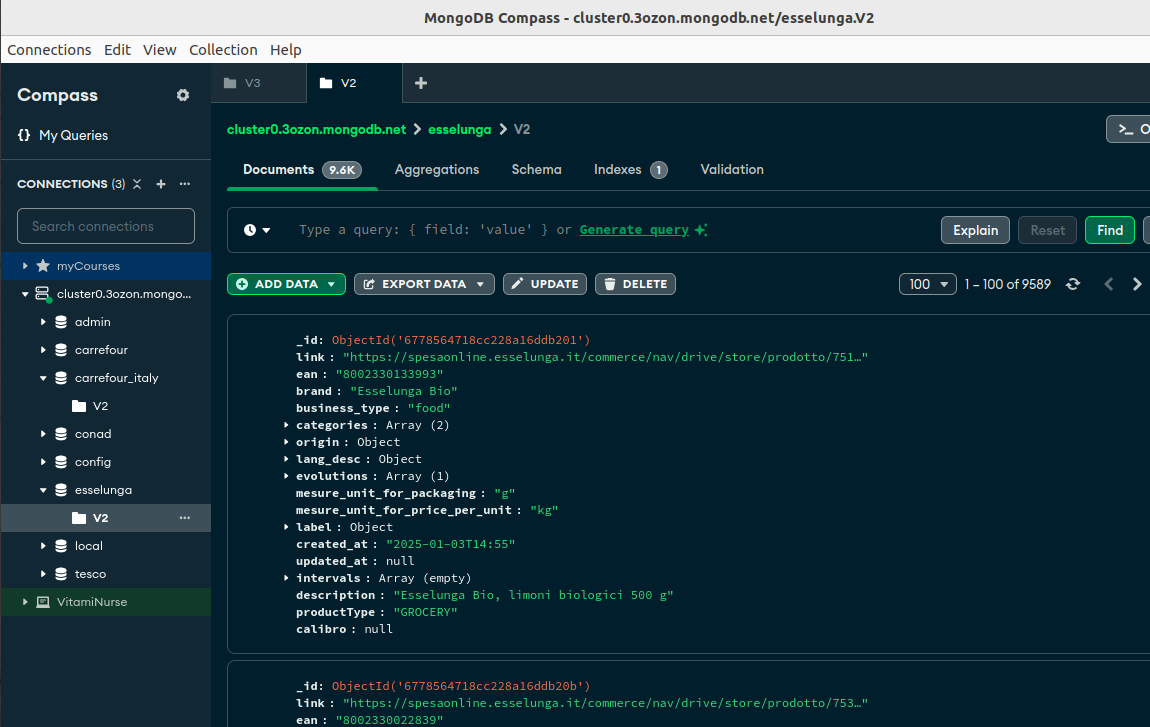
\includegraphics[scale=0.35]{images/load_data.png}
    \caption{Load products for each market in MongoDB} 
    \label{fig:load_data_mongo}
\end{figure}
\end{center}

\subsection{Optimized Vector Store in ChromaDB}
Following data transformation, a light copy of the users and products collections is generated, containing only essential attributes such as the product name, category, and nutritional information. This refined database is then embedded and stored in ChromaDB, enabling efficient semantic search and powering the recommendation and conversational systems.



\subsection{Dual-database architecture}
 
Following data transformation, a refined copy of the users and products
collections is generated, containing only essential attributes such as
the product name, category, and nutritional information. In order to
optimize retrieval and analysis, this database is then embedded and
stored in ChromaDB. This vector database enables similarity search,
allowing the application to easily access and utilize it for further analysis or recommendation.

The following tools were employed to facilitate data management, embedding generation, and semantic retrieval:
\begin{itemize}[label=$\bullet$]
    \item \textbf{MongoDB Atlas}: A cloud-hosted NoSQL database service for the efficient storage and management of structured data, offering scalability and ease of deployment in distributed environments.
    \item \textbf{PyMongo}: A robust Python library that enables seamless programmatic interaction with MongoDB instances, supporting operations such as data insertion, querying, and updates.
    \item \textbf{MongoDB Compass}: An intuitive graphical user interface tool for exploring MongoDB collections and visualizing data.
    \item \textbf{ChromaDB}: An open-source vector database optimized for high-dimensional embeddings and enabling efficient similarity searches, particularly suited for semantic querying tasks.
    \item \textbf{SentenceTransformers}: A Python-based library that uses transformer models to generate dense vector representations (embeddings) from textual input.
\end{itemize}


\section{Web scraping}
\subsection{Web Scraping Process}
The web scraping process took place in several successive stages to ensure efficient information extraction:
\begin{itemize}
    \item \textbf{Page Access:}
    Using Selenium, we automated access to the various product pages by simulating clicks and navigation between departments, categories, and subcategories.
    \item \textbf{Information Extraction:} Once the page loaded, specific information (product name, description, price, images, and storage instructions) was extracted by analyzing the HTML structure. Particular care was taken to retrieve relevant data, filtering out unnecessary elements.
    \item \textbf{Error Handling:} During scraping, error handling mechanisms were implemented to manage potential page blocks, access restrictions, or changes to the page structure.
\end{itemize}

The main challenge  we encountered is Anti-bot management . And we can overcome this problem by using solutions like random delays, proxy rotation, and user agent switching.


\subsection{used tools in web scraping}
We have to relied on a complementary set of tools tailored to the diversity of data sources and formats encountered.
\begin{itemize}
    \item \textbf{Selenium:} was used to automate interactions with dynamic web pages, cookie banners or  AJAX scenarios where data loaded via AJAX is not immediately available in the DOM.
    \item \textbf{BeautifulSoup:}  enabled fast and efficient extraction of information from static HTML content.
    \item \textbf{cURL and Requests :} To interact with REST APIs, cURL and Python’s Requests library allowed for simple HTTP requests, sometimes requiring authentication or specific parameters. 
\end{itemize}

\subsection{Combine scraping tools}
To scrape Esselunga's Italian market, we combine Selenium, BeautifulSoup, and API requests for efficiency. First, a \textbf{Selenium} script navigates product categories, scrolls to load all items, and collects individual product links (see Figure \ref{fig:get products links}).
\begin{figure}[H]
            \centering
            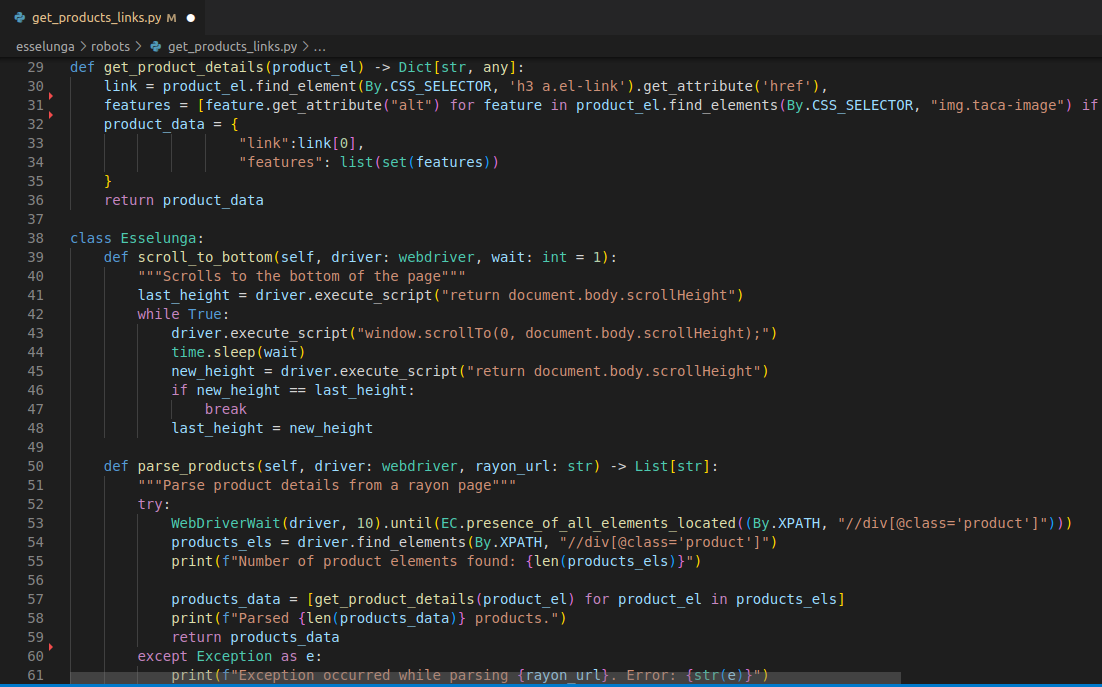
\includegraphics[scale=0.42]{images/get_products_links.png}
            \caption{get products links} 
            \label{fig:get_products_links}
\end{figure}

Once the product links have been collected. A second script then uses the \textbf{requests} library to rapidly fetch product data directly from the API. \textbf{BeautifulSoup} parses the HTML, avoiding the slower process of loading each page with Selenium.

For robustness and speed, the script includes a retry mechanism for errors and uses a \textbf{ThreadPoolExecutor} for concurrent requests. This approach successfully retrieved data for over 9,000 products in under three minutes as shown in Figure \ref{fig:all_data_scanner}.

\begin{figure}[H]
            \centering
            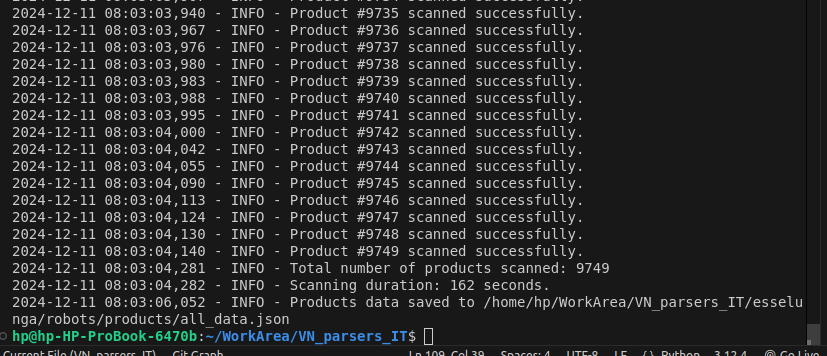
\includegraphics[scale=0.42]{images/all_data_scanner.png}
            \caption{all data scanner} 
            \label{fig:all_data_scanner}
\end{figure}




\newpage
\section{Nutrition prediction}
In the VitamiNurse project, automated completion of missing nutritional values represents a critical challenge. The primary data source relies on web scraping, which frequently yields products with incomplete or missing nutritional information. This section details the development and evolution of the machine learning model Nutri-pred-v1, specifically designed to address this need by automatically predicting nutritional values of food products from their names and textual descriptions.

\subsection{Training data}

 The Open Food Facts (OFF) allows us to either download the latest complete dataset in both CSV and JSON formats. It is  a collaborative and open-access database that contains information of more than 3.8 million food products. Because of its extensive size (11.4 GB) and the high dimensionality of the data, it is essential to optimize memory usage during data preprocessing. 
  An effective and widely used technique in data science consists of loading only the columns needed for training the model. This selective loading approach significantly reduces memory consumption and processing time.

\par As shown below, only the columns required for training are loaded from the dataset:

\begin{center}
\begin{figure}[H]
    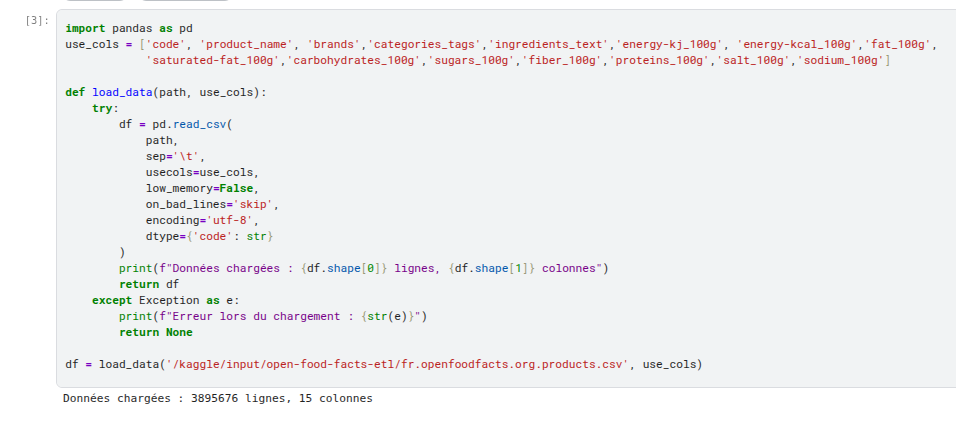
\includegraphics[scale=0.44]{images/load_dataset.png}
    \caption{The selective loading approach} 
    \label{fig:load_dataset}
\end{figure}
\end{center}

\subsection{Exploring dataset problems}
Because of the collaborative nature of the dataset, many problems can be encountered. It require substantial cleaning and preprocessing efforts in order to ensure reliability of our data.
These problems include :
\begin{itemize}
\item \textbf{Missing Values:} Many entries have incomplete nutritional profiles, which affects the ability to use them for training ML models.
\item \textbf{Inconsistent and Erroneous Values:} Some fields contain inconsistent or obviously erroneous values due to unit or user input errors .

\item \textbf{Negative Values:} Several nutritional values are negative, which is physiologically unrealistic.
\end{itemize}

\begin{center}
\begin{figure}[H]
    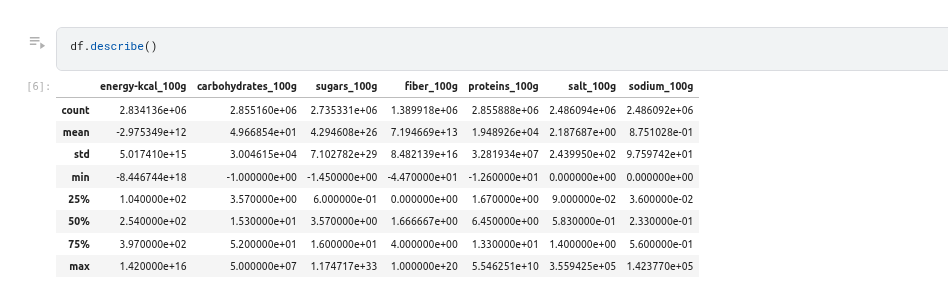
\includegraphics[scale=0.55]{images/statistics.png}
    \caption{Explore data statistics} 
    \label{fig:data_statistics}
\end{figure}
\end{center}

\subsection{Feature Selection Strategy}
The feature selection strategy for our high-dimensional nutritional dataset integrates established machine learning principles to enhance model robustness. This approach, combining correlation-driven dimensionality reduction, missing  informed-data exclusion, and unit consolidation, optimizes predictive performance while preserving essential information. This step is important to ensure effective model training while preserving critical nutritional information.

\subsubsection{Correlation-Driven Feature Exclusion}
To mitigate redundancy and numerical instability, we exclude features exhibiting near-perfect correlation. Following Guyon and Elisseeff (2003) \cite{guyon2003}, the feature energy-kJ\_100g is removed due to its perfect negative correlation ($r \approx -1$) with energy-kcal\_100g. Including both variables provides no additional predictive information and risks numerical instability in model training due to multicollinearity. Instead, we retain energy-kcal\_100g and leverage the thermodynamic conversion factor:
$$1~\mathrm{kcal} = 4.184~\mathrm{kJ}$$


This expression is used to derive energy-kJ\_100g post-training, ensuring computational stability and preserving predictive accuracy.

% Creating the table for nutritional ranges
\begin{center}
\begin{figure}[H]
    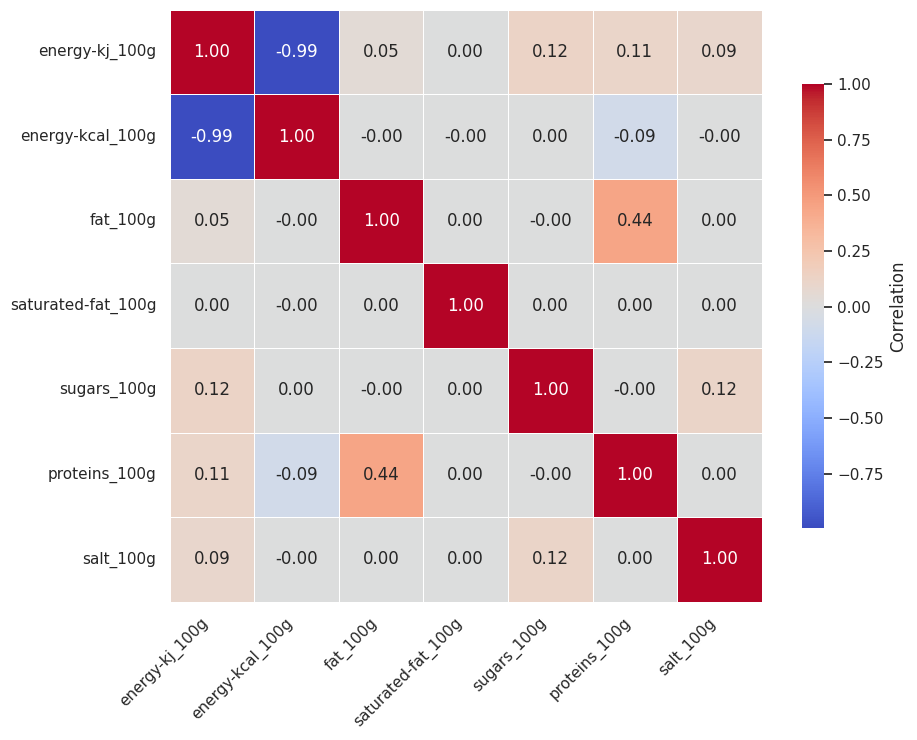
\includegraphics[width=0.9\textwidth]{images/correlation_matrix.png}
    \caption{Correlation matrix} 
    \label{fig:Correlation_matrix}
\end{figure}
\end{center}


\subsubsection{Handling Missing Data}
To address the challenge of missing data, we adopt a selective retention. Features with high missingness, such as energy-kJ  (missing >86 \%) and fiber (missing >52 \%), are excluded in order to preserve data integrity and avoid imputation bias. 
\par In contrast, the other nutritional features (energy-kcal,
fat, carbohydrates, and proteins) are retained due to their low missingness rates  ($<$ 3.3\%) and critical role in nutritional modeling \cite{stoian2020machine}.


This selective
retention ensures a robust and representative set of features in order to guarantee an effective model training.

\begin{center}
\begin{figure}[H]
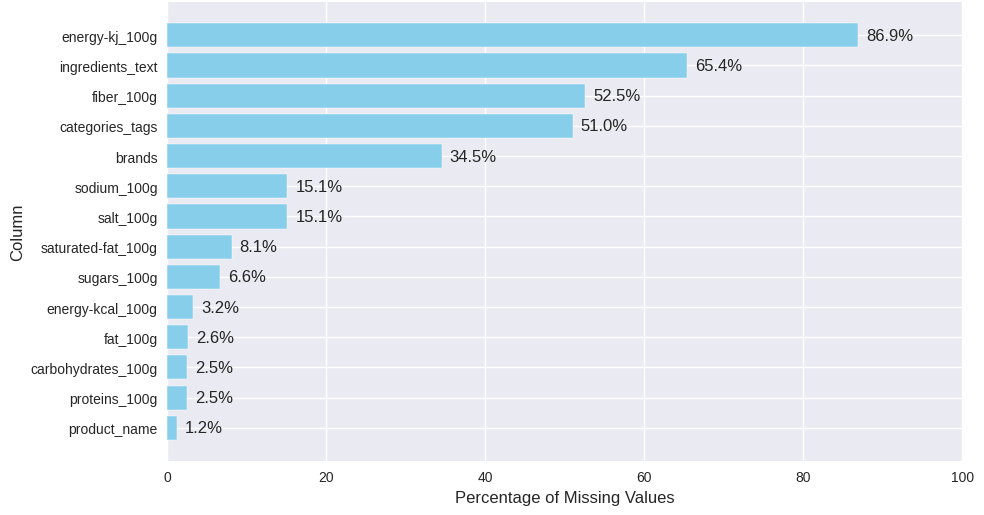
\includegraphics[scale=0.35]{images/missing_values.png}
\caption{Proportion of missing values} 
\label{fig:missing_values}
\end{figure}
\end{center}

\newpage
\subsection{Data processing and cleaning}
\subsubsection{Initial Dataset Overview}
The initial dataset comprised 3,800,000 products. After preprocessing and cleaning, the dataset was reduced to 2,225,014 products, ensuring:
\begin{itemize}
    \item Complete textual descriptions for all products.
    \item Non-null and plausible nutritional values.
    \item Homogenized units for consistency across the dataset.
\end{itemize}

\subsubsection{Preprocessing Steps}
The preprocessing phase was designed to ensure data consistency and compatibility. In order to maintain data integrity, text cleaning was done first. This included the removal of special characters, normalize text case to ensure uniformity , and systematic process missing or inconsistent text fields . Text descriptions were then vectorized using the Term Frequency-Inverse Document Frequency (TF-IDF) approach in order to extract features. This process transformed the text data into numerical representations, limiting the feature set to a maximum of 12,000 features  to optimize computational efficiency and model performance. This choice will be proved later in the Hyperparameter Tuning step ~\ref{tab:max_features_values}.

\subsubsection{Filtering implausible nutritional values}

This filtering step was implemented in order to remove entries with implausible nutritional values, such as negative calories or excessive amounts of nutrients. These errors can distort  the performance any machine learning model. We defined plausible nutritional ranges for each nutrient per 100g of product. These thresholds reflect chemically realistic limits. 
For example,  900 kcal represents the upper physiological limit for energy content in food composed solely of fat, such as oils. This theoretical maximum energy is calculated based on the Atwater general factor system that includes energy values of 4 kcal per gram (17 kJ/g) for protein, 4 kcal/g for carbohydrates and 9 kcal/g (37 kJ/g) for fat \cite{huel_energy_calculation}.

Thus the total energy content per 100 grams can be estimated using the following formula:

$$
\text{Energy (kcal/100g)} = 4 \times (\text{g carbs}) + 4 \times (\text{g proteins}) + 9 \times (\text{g fats})
$$

The theoretical maximum energy density is reached when a product consists entirely of fat, as it yields the highest caloric value per gram. In this case, the energy content is:

\[
\text{Energy} = 9 \times 100 = 900 \text{ kcal/100g}
\]


The process then continues with all the other macronutrients like it is illustrated in the provided table to retain only nutritionally realistic entries.



% Creating the table for nutritional ranges
\begin{table}[H]
\centering
\caption{Plausible Nutritional Ranges for Data Validation in product Composition per 100g)}
\resizebox{0.9\textwidth}{!}{%
\begin{tabular}{@{}lcp{10cm}@{}}
\toprule
\textbf{Nutrient} & \textbf{Plausible Range} & \textbf{Scientific Rationale and Validation Criteria} \\
\midrule
Energy & 0--900 kcal & Energy content is derived from the Atwater system by employing the 4-9-4 method: carbohydrates, proteins and fats. The theoretical maximum of $\sim$900 kcal/100g occurs in pure fats like oils. \\  \\
Carbohydrates & 0--100 g & Includes sugars, starches, and dietary fiber, expressed as a mass fraction. Pure carbohydrate sources like sugar and starch may approach 100 g/100g, constrained by total mass . \\ \\
Total Fat & 0--100 g & Represents all lipid fractions. Pure fats like olive oil and butter may reach 100 g/100g, validated by gravimetric methods like Soxhlet extraction. \\ \\
Saturated Fat & 0--100 g & A subset of total fat, limited by total fat content. Pure saturated fat sources such as coconut oil may reach 100 g/100g, quantified via gas chromatography . \\ \\
Sugars & 0--100 g & Includes mono- and disaccharides. Pure sugar products (e.g., sucrose, honey) may reach 100 g/100g. \\ \\
Proteins & 0--90 g & Limited by food matrix composition. High-protein foods like whey protein and dried meat may approach 90 g/100g, quantified by Dumas methods \cite{moore2022}. \\ \\
Salt & 0--30 g & Constrained by sensory acceptability and public health recommendations outlined by the World Health Organization (WHO) regarding sodium intake \cite{who2012}. \\
\bottomrule
\end{tabular}
}
\label{tab:nutritional_ranges}
\end{table}


\subsubsection{Data cleaning}
To ensure data integrity and eliminate redundancy, we identified and removed 1604 fully duplicated rows in the dataset to ensure that each product instance is unique.
\par Additionally, since the product name is a critical textual feature for nutritional prediction, we discarded 23,740 rows with missing values in the product\textunderscore name field to guarantee meaningful and consistent textual representations. For the training process, only the product\textunderscore name field was vectorized using the TF-IDF (Term Frequency–Inverse Document Frequency) approach to extract relevant textual features for modeling.

\begin{figure}[H]
\centering
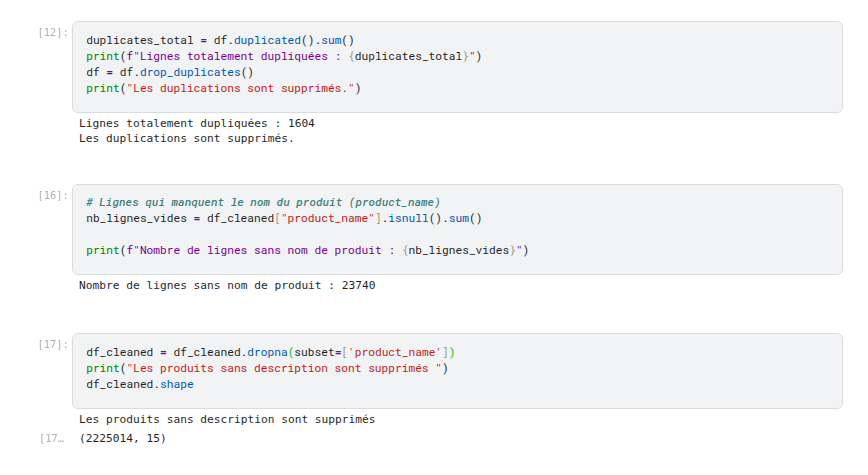
\includegraphics[scale=0.44]{images/data_cleaning.png}
\caption{Removal of duplicates and rows with missing product names.}
\label{fig:data_cleaning}
\end{figure}

\subsection{Sampling and Training Set Construction}
A stratified random sample of 10\% of the dataset (222,501 products) was selected to perform model experimentation and hyperparameter tuning. The target variables were the following nutritional attributes: energy (kcal), fat, saturated fat, carbohydrates, sugars, proteins, and salt.
Entries with missing values in any of these target variables were removed to ensure reliable supervision during training.

\subsection{TF-IDF Hyperparameter Optimization}
A machine learning pipeline was developed, integrating a Term Frequency-Inverse Document Frequency (TF-IDF) Vectorizer with a multi-output regression model to predict nutritional attributes from the product\_name, aligning with established natural language processing practices.
\par To optimize performance, a grid search with 3-fold cross-validation was conducted to determine the optimal \texttt{max\_features} parameter for the TF-IDF Vectorizer, ensuring robust model evaluation \cite{hastie2009elements}. The following configurations were evaluated:

\begin{itemize}
    \item \textbf{Base Regressor}: Linear Regression was selected as the foundational model for the multi-output regression task, leveraging its simplicity and effectiveness in high-dimensional settings, consistent with the dataset's characteristics.
    \item \textbf{Hyperparameter Tuning}: The \texttt{max\_features} parameter of the TF-IDF Vectorizer was tuned over different values ranging from 500 to 15000 , following standard approaches for optimizing feature selection in text-based nutritional prediction \cite{aionlinecourse2025}.
\end{itemize}


\begin{table}[H]
\centering
\caption{Comparison of Mean Absolute Error (MAE) for Different \texttt{max\_features} Values}
\begin{tabular}{cS[table-format=5.0]S[table-format=2.4]S[table-format=1.4]}
\toprule
{Fold} & {\texttt{max\_features}} & {MAE} & {Standard Deviation} \\
\midrule
1 & 500 & 23.6168 & 0.0169 \\
2 & 1000 & 22.1044 & 0.0069 \\
3 & 2000 & 20.6975 & 0.0255 \\
4 & 3000 & 20.0193 & 0.0029 \\
5 & 5000 & 19.3171 & 0.0131 \\
6 & 6000 & 19.1467 & 0.0058 \\
7 & 7000 & 19.0157 & 0.0149 \\
8 & 8000 & 18.9249 & 0.0086 \\
9 & 9000 & 18.8800 & 0.0109 \\
10 & 10000 & 18.8278 & 0.0037 \\
11 & 12000 & 18.7647 & 0.0193 \\
12 & 14000 & 18.7665 & 0.0222 \\
13 & 15000 & 18.7676 & 0.0248 \\
\midrule
\multicolumn{2}{l}{\textbf{Best Parameter}} & \multicolumn{2}{l}{\texttt{max\_features} = 12000} \\
\multicolumn{2}{l}{\textbf{Best MAE}} & \multicolumn{2}{l}{18.7647} \\
\bottomrule
\end{tabular}
\label{tab:max_features_values}
\end{table}

\vspace{0.4cm}
\par As shown in the previous table the grid search identified the optimal configuration with \texttt{max\_features = 12000}. By achieving a Mean Absolute Error (MAE) of 18.76,it demonstrates effective predictive performance for the nutritional attributes. While increasing the number of features consistently improved accuracy, gains became marginal beyond 12000, suggesting this value offers a good balance between complexity and performance.




\subsection{Models Evaluation}
\par This step we evaluate the effectiveness of various machine learning algorithms for predicting nutritional values, a comprehensive comparative analysis was conducted. This study assessed the performance of multiple regression models, including K-Nearest Neighbors (KNN), Linear Regression, CatBoost, LightGBM, XGBoost, and Random Forest.
% Including figure for model comparison
\begin{figure}[H]
    \centering
    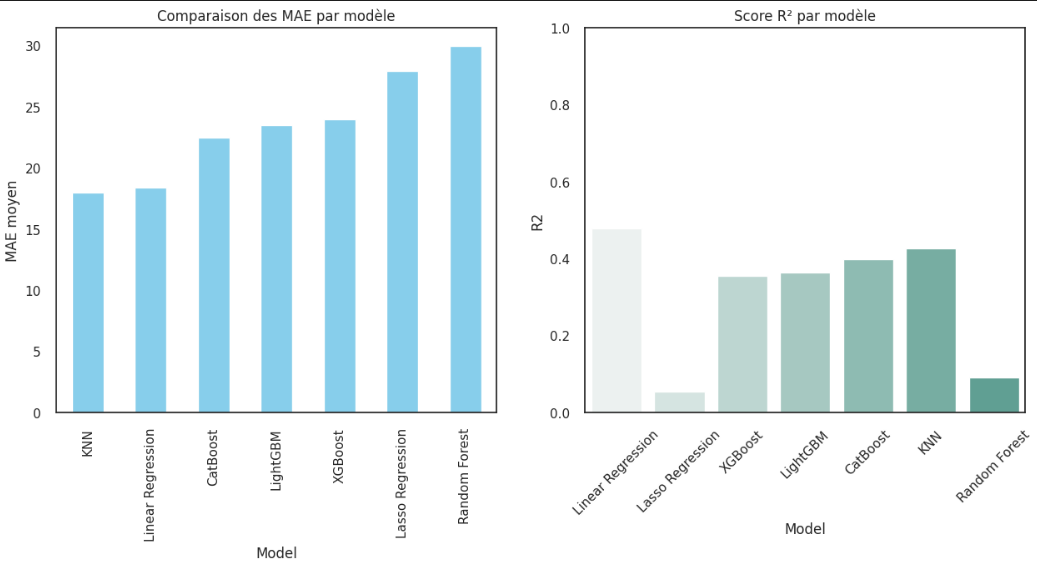
\includegraphics[width=0.9\linewidth]{images/mae_r2_comparison.png}
    \caption{Comparison of Mean Absolute Error (MAE) and \(R^2\) across regression models.}
    \label{fig:model_comparison}
\end{figure}

The performance of each model was quantified using two key metrics: Mean Absolute Error (MAE) and coefficient of determination ($R^2$) that offer critical insights into model accuracy and explanatory power. The results are summarized in the table~\ref{tab:model_results}, with MAE and \(R^2\) values for each algorithm.


\begin{table}[H]
    \centering
    \caption{Performance metrics of regression models}
    \begin{tabular}{lcc}
        \toprule
        \textbf{Model} & \textbf{MAE} & \textbf{\(R^2\)} \\
        \midrule
        K-Nearest Neighbors & 17.939 & 0.427 \\
        Linear Regression & 18.396 & 0.478 \\
        CatBoost & 22.472 & 0.397 \\
        LightGBM & 23.499 & 0.364 \\
        XGBoost & 23.948 & 0.354 \\
        Lasso Regression &  27.933 & 0.055 \\
        Random Forest & 29.955 & 0.090 \\
        \bottomrule
    \end{tabular}
\end{table}

\newpage
\subsection{Model selection}
 The K-Nearest Neighbors (KNN) model achieved the lowest MAE of 17.94, indicating high predictive accuracy with minimal average deviation between predicted and actual values. Its \(R^2\) of 0.427, while reasonable, is slightly lower than Linear Regression’s 0.478, which captures a marginally higher proportion of variance. 
 \par Other models, including CatBoost , LightGBM , XGBoost , and Random Forest , exhibited higher errors and lower explanatory power, with Random Forest performing notably poorly (MAE: 29.95, \(R^2\): 0.090), likely due to overfitting in the high-dimensional TF-IDF feature space. Given the priority of minimizing prediction errors for nutritional analysis. KNN’s superior MAE makes it the preferred model, despite its slightly lower \(R^2\). 

\subsection{Model architecture}
Trained on a large dataset of 2.2 million products and demonstrating strong generalization with satisfactory accuracy, the model Nuti-prd-v1 utilized a MultiOutputRegressor based on KNeighborsRegressor (n\_neighbors=5, n\_jobs=-1). It is selected after comparative evaluation of multiple multi-output regression algorithms trained on the complete Open Food Facts dataset. This configuration, designated Nutri-pred-v1, minimized the mean absolute error (MAE) on nutritional variables.

\begin{itemize}
    \item \textbf{Input}: TF-IDF vectors (12,000 features) derived from product names and descriptions
    \item \textbf{Output}: Predictions for 7 nutritional variables
    \item \textbf{Energy calculation}: energy\_kj\_100g = energy\_kcal\_100g × 4.184
    \item \textbf{KNN rationale}: Selected for its capacity to capture nonlinear relationships in high-dimensional TF-IDF space, demonstrating superior MAE performance among tested models
\end{itemize}


\subsection{Model Evaluation}
The K-Nearest Neighbors (KNN) model achieved the lowest MAE of 18.36, indicating high predictive accuracy with minimal average deviation between predicted and actual values. Its R2 of 0.417, while reasonable, is slightly lower than Linear Regression’s 0.457, which captures a marginally higher
proportion of variance.
Other models, including CatBoost , LightGBM , XGBoost , and Random
Forest , exhibited higher errors and lower explanatory power, with Random
Forest performing notably poorly (MAE: 29.77, R2 : 0.105), likely due to
overfitting in the high-dimensional TF-IDF feature space. Given the priority
of minimizing prediction errors for nutritional analysis. KNN’s superior MAE
makes it the preferred model, despite its slightly lower R2 .
\subsection{Prediction}
\begin{itemize}
    \small
    \item Link: \href{https://www.auchan.fr/auchan-creme-fraiche-epaisse-entiere-30-mg/pr-C1177977}{AUCHAN Thick Whole Cream}
    \item Textual description: AUCHAN Crème fraîche épaisse entière 30\%MG
\end{itemize}
\begin{table}[H]
    \centering
    \caption{Nutritional prediction}
    \resizebox{0.95\textwidth}{!}{%
    \begin{tabular}{lccc}
        \toprule
        \textbf{Nutrient} & \textbf{Actual Value } & \textbf{Predicted Value } & \textbf{Absolute Error} \\
        \midrule
        Energy (kcal/100g) & 291 & 290.4 & 0.6 \\
        Energy (kJ/100g) & 1200 & 1215.03 & 15.03 \\
        Fat (g/100g) & 30 & 30.04 & 0.04 \\
        Saturated Fat (g/100g) & 19 & 20.24 & 1.24 \\
        Carbohydrates (g/100g) & 2.9 & 2.72 & 0.18 \\
        Sugars (g/100g) & 2.9 & 2.7 & 0.2 \\
        Proteins (g/100g) & 2.4 & 2.34 & 0.06 \\
        Salt (g/100g) & 0.07 & 0.08 & 0.01 \\
        \bottomrule
    \end{tabular}
    }
\end{table}

\begin{itemize}
    \small
    \item Local MAE: ~0.33
    \item Accuracy: Highly satisfactory
\end{itemize}
\thispagestyle{fancy}
\subsection{Model Deployment}
This model is deployed as \textbf{Nutri-Pred-v1}, a high-precision model leveraging its lower MAE for applications requiring maximum predictive accuracy, such as detailed nutritional analysis.

The deployment infrastructure includes:
\begin{itemize}
    \item \textbf{Infrastructure}: Model optimized for rapid execution < 0.5 s/prediction (0.2 s/batch)
    \item \textbf{Model export}: The model is exported via joblib for easy integration
    \item \textbf{REST API}: A FastAPI-based REST API enables nutritional predictions for both individual products and batch processing
    \item \textbf{User interface}: A Gradio interface deployed on Hugging Face
facilitates interactive testing\footnotemark.
\footnotetext{\url{https://huggingface.co/spaces/bellgacem/Nutri-pred-v1}}
\end{itemize}


\begin{figure}[H]
    \centering
    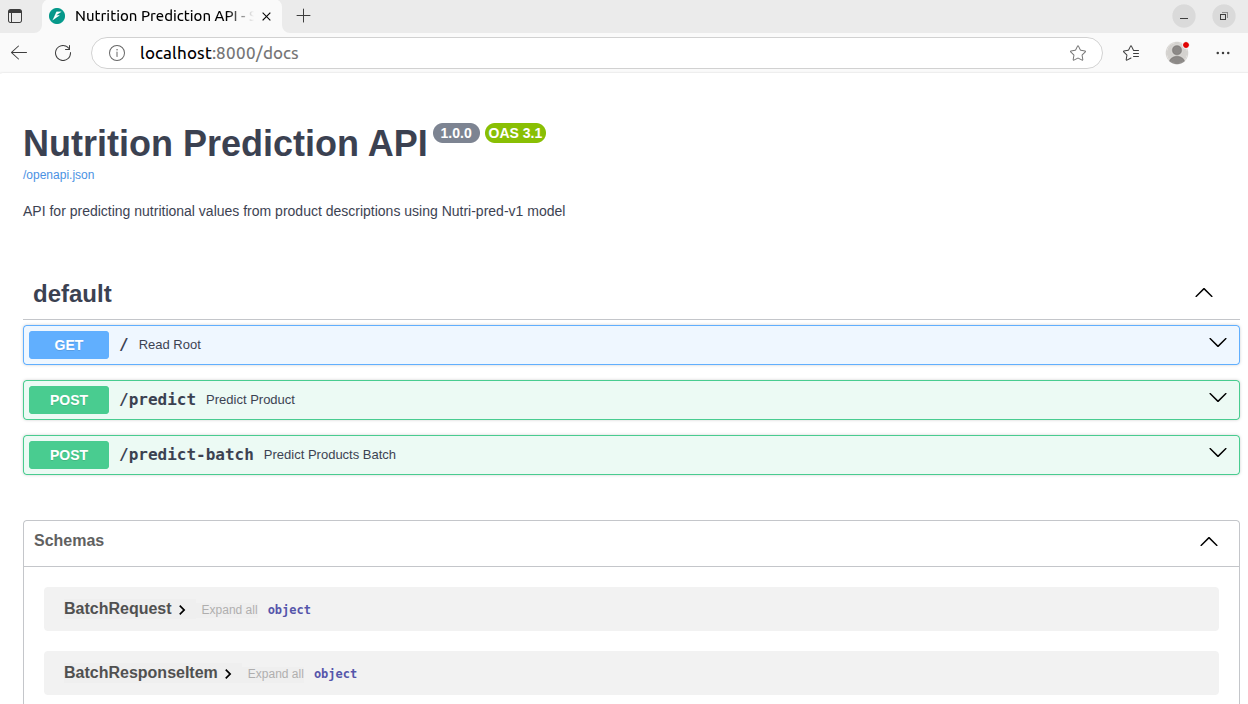
\includegraphics[width=0.90\textwidth]{images/Nutri-pred_fast_API.png}
    \caption{FastAPI endpoint for predicting nutritional values.}
    \label{fig:fastapi-endpoint}
\end{figure}

\vspace{1cm}
The deployment architecture ensures low-latency predictions and supports both local and cloud execution environments. The combination of RESTful access and interactive UI enhances accessibility for developers and non-technical users of this model.


\begin{figure}[H]
    \centering
    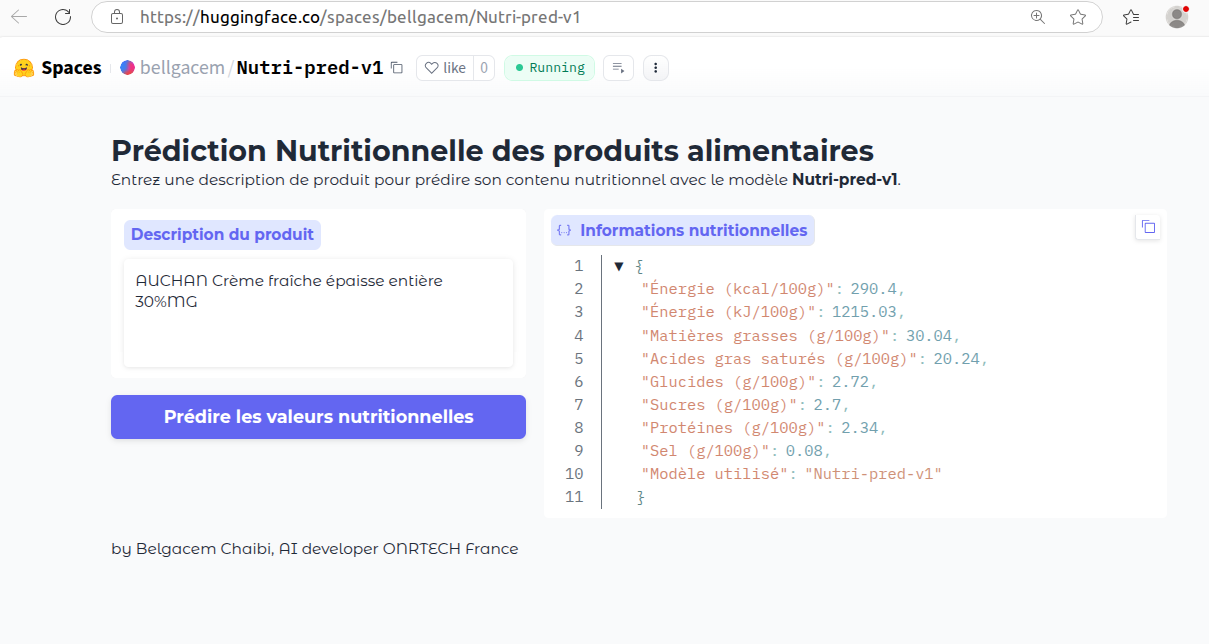
\includegraphics[width=0.90\textwidth]{images/Nutri-pred_Huggingface.png}
    \caption{Gradio interface for Nutri-Pred-v1 hosted on Hugging Face Spaces.}
    \label{fig:gradio-ui}
\end{figure}


\section*{Conclusion}
In conclusion, we can provide a robust foundation for ingesting and processing data from multiple platforms by building a robust data pipeline and the Nutri-Pred-v1 model. This ML model enhances the pipeline’s functionality by delivering highly accurate predictions of nutritional values for products lacking such information.
 Furthermore, to optimize semantic search and enable real-time personalized recommendations, we implemented a vector database for efficient data storage and retrieval within the AI assistant and recommendation engine.


 